\documentclass[10pt,a4paper]{amsart}
\usepackage[margin=19mm]{geometry}
\usepackage{amsmath,amssymb,mathtools}
\usepackage[scr=rsfs,cal=euler]{mathalfa}
\usepackage{xfrac}
\usepackage[unicode,hidelinks,bookmarks=false]{hyperref}
\newcommand{\ie}{i.e.\ }
\newcommand{\cf}{cf.\ }
\newcommand{\resp}{respectively\ }
\newcommand{\Subsection}{\subsection}
\providecommand{\nobreakdash}{\nobreak\hbox{-}}
\setlength{\emergencystretch}{2em}
\multlinegap0pt
\usepackage{tikz}
\usepackage[all]{xy}
\usepackage{mathtools}
\usepackage{amssymb}
\usepackage{enumerate}
\usepackage{caption}
\usepackage{algorithm}\usepackage{algpseudocode}
\newtheorem{lem}{Lemma}
\newtheorem{claim}{Claim}
\newcommand{\U}{ X}
\newcommand{\pU}{\partial{  X}}
\newcommand{\proj}{\textbf{d}}
\title{Genericity of sublinearly Morse directions in general metric spaces}
\author{Yulan Qing, Wenyuan Yang}
\date{Source: arXiv:2404.18762v2 (CC BY 4.0)}
\begin{document}
\maketitle

\noindent\emph{Source and licence.} Genericity of sublinearly Morse directions in general metric spaces. Version arXiv:2404.18762v2 (CC BY 4.0), distributed by arXiv under the Creative Commons Attribution 4.0 International licence, http://creativecommons.org/licenses/by/4.0/, as recorded in the arXiv licence metadata for this exact version and shown on the abstract page https://arxiv.org/abs/2404.18762v2. Full licence notice: \texttt{licenses/arxiv-2404.18762-CC-BY-4.0.txt}.\par\smallskip

\noindent\textit{Editorial scope.} Counted unit: the article's lem RegContrRayClass (source0.tex lines 1283--1287). The article's complete original proof of it is delivered with it (source0.tex lines 1288--1387, one \texttt{proof} environment of 100 lines). No mathematics is written, repaired or re-derived: the statement and the proof are the article's own lines, in the article's own notation, and no retained line is substituted or re-flowed.  Retained uncounted as the source-local context the proof needs: lines 1203--1207; lines 1259--1263.  Nothing was omitted from any retained span, so the package carries no omission record.  No retained line contains a citation, so the wrapper carries no bibliography and no bibliography entry.  The retained lines contain the article's own diagram code, which the wrapper typesets with the standard tikz packages; no image file is delivered and the package declares no asset dependency.  Editorial formatting only, in addition: an AMS \texttt{amsart} preamble that restates the article's own declarations and macros used by the retained lines, namely the environments \texttt{lem}, \texttt{claim} on separate counters, together with the standard packages those lines need.  The retained environments print in this document as Lemma 1, Claim 1 in order of appearance, whereas the article prints the same items with the numbering of its own full document.  The complete native source of the article as distributed in the arXiv e-print for this exact version is bundled unchanged as \texttt{sources/158333/source0.tex}.
\begin{equation}\label{rclosetopEQ}
t \in [s-L/2 , s+L/2]
\qquad\Longrightarrow \qquad
d(\gamma(t), p) \leq r.    
\end{equation}

\begin{lem}\label{close barriers in two geodesics}
For any $r\ge C,M>0$ there exist $\hat r=\hat r(r,C,M), L_0=L_0(r,C,M)>0$ with the following property.

Assume that $\alpha$ and $\beta$ are two geodesics with $d(\alpha^-,\beta^-), d(\alpha^+,\beta^+)\le M$. Let $p$ be a $C$-contracting segment with length at least $L_0$. If  $d(p^-,\alpha),d(p^+,\alpha)\le r$, then $d(p^-,\beta),d(p^+,\beta)\le \hat r$.    
\end{lem}

\begin{lem}\label{RegContrRayClass}
Given constants $r\ge C>0$, there exist $\hat r=\hat r(r,C), L_0=L_0(r,C)$ with the following property.

Given $L\ge L_0$ and $\theta\in (0,1]$, let $\gamma$  be an $(r, C, L)$--contracting  geodesic ray  at $\theta$–frequency starting at a point $o\in \U$. Assume that the terminal $[\cdot]$-class $[\gamma^+]$ of  $\gamma$ is non-pinched. Then any geodesic ray from $o$ ending at $[\gamma^+]$ in $\pU$ is $(\hat r, C, L)$--contracting   at $\theta$–frequency.
\end{lem}

\begin{proof}
Throughout the proof, all constants depend only on $r$ and $C$. 
By assumption, let  $p_n$ be a sequence of the $C$--contracting geodesic segments  for $\gamma$ witnessing the property (\ref{rclosetopEQ}). Excising subsegments from $p_n$ with length $L$ if necessary, we may assume that $\{p_n: n\ge 1\}$ is    escaping and each $p_n$ has length  $L$. 

Let $x_n,y_n\in \gamma$ be the entry and exit points of $\gamma$ in $N_r(p_n)$, so the endpoints of $p_n$ being contained in $N_r(\gamma)$ yields $$d(x_n,y_n)\ge \ell(p_n)-2r\ge L-2r$$ Let $x_n', y_n'\in p_n$ so that $d(x_n,x_n'),d(y_n,y_n')\le r$. The first paragraph in the proof of Lemma \ref{close barriers in two geodesics} proves $d(x_n',p_n^-),d(y_n',p_n^+)\le 4r$. That is, the projection of  $x_n$ (resp. $y_n$) to $p_n$ lies in the $4r$-neighborhood of $p_n^-$ (resp. $p_n^+$). By the $C$-contracting property, $[o,x_n]_\gamma$ projects to $p_n$  as a subset with diameter at most $C$, which thus is  $(C+4r)$-close to $p_n^-$. Similarly, if $u$ is a point  on $\gamma$ with $d(o,u)\ge d(o,y_n)$, the projection of $[y_n,u]_\gamma$ to $p_n$ is $(C+4r)$-close to $p_n^+$. 

\begin{figure}
    \centering


\tikzset{every picture/.style={line width=0.75pt}} %set default line width to 0.75pt        

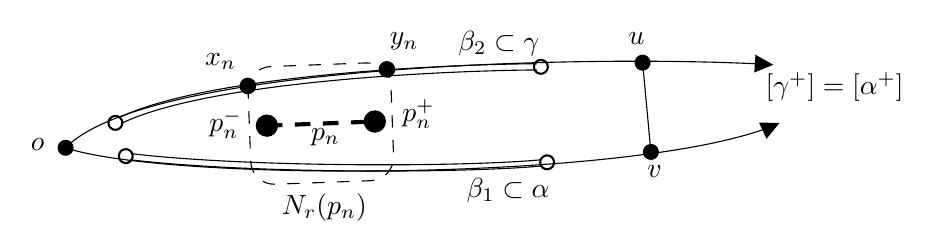
\begin{tikzpicture}[x=0.75pt,y=0.75pt,yscale=-1,xscale=1]
%uncomment if require: \path (0,300); %set diagram left start at 0, and has height of 300

%Curve Lines [id:da45971128384035875] 
\draw    (100,121) .. controls (139.6,80.41) and (355.62,76.08) .. (438.53,80.85) ;
\draw [shift={(441,81)}, rotate = 183.53] [fill={rgb, 255:red, 0; green, 0; blue, 0 }  ][line width=0.08]  [draw opacity=0] (8.93,-4.29) -- (0,0) -- (8.93,4.29) -- cycle    ;
%Curve Lines [id:da9983642169841976] 
\draw    (100,121) .. controls (150.49,137.83) and (379.36,137.02) .. (442.15,109.83) ;
\draw [shift={(444,109)}, rotate = 154.98] [fill={rgb, 255:red, 0; green, 0; blue, 0 }  ][line width=0.08]  [draw opacity=0] (8.93,-4.29) -- (0,0) -- (8.93,4.29) -- cycle    ;
\draw [shift={(100,121)}, rotate = 18.43] [color={rgb, 255:red, 0; green, 0; blue, 0 }  ][fill={rgb, 255:red, 0; green, 0; blue, 0 }  ][line width=0.75]      (0, 0) circle [x radius= 3.35, y radius= 3.35]   ;
%Straight Lines [id:da313503894956524] 
\draw    (378,80) -- (382,123) ;
\draw [shift={(382,123)}, rotate = 84.69] [color={rgb, 255:red, 0; green, 0; blue, 0 }  ][fill={rgb, 255:red, 0; green, 0; blue, 0 }  ][line width=0.75]      (0, 0) circle [x radius= 3.35, y radius= 3.35]   ;
\draw [shift={(378,80)}, rotate = 84.69] [color={rgb, 255:red, 0; green, 0; blue, 0 }  ][fill={rgb, 255:red, 0; green, 0; blue, 0 }  ][line width=0.75]      (0, 0) circle [x radius= 3.35, y radius= 3.35]   ;
%Straight Lines [id:da9632229487773224] 
\draw [line width=1.5]  [dash pattern={on 5.63pt off 4.5pt}]  (196.98,110.34) -- (248.98,108.34) ;
\draw [shift={(248.98,108.34)}, rotate = 357.8] [color={rgb, 255:red, 0; green, 0; blue, 0 }  ][fill={rgb, 255:red, 0; green, 0; blue, 0 }  ][line width=1.5]      (0, 0) circle [x radius= 4.36, y radius= 4.36]   ;
\draw [shift={(196.98,110.34)}, rotate = 357.8] [color={rgb, 255:red, 0; green, 0; blue, 0 }  ][fill={rgb, 255:red, 0; green, 0; blue, 0 }  ][line width=1.5]      (0, 0) circle [x radius= 4.36, y radius= 4.36]   ;
%Rounded Rect [id:dp09550547549508426] 
\draw  [dash pattern={on 4.5pt off 4.5pt}] (187.92,93.61) .. controls (187.69,87.34) and (192.58,82.07) .. (198.84,81.84) -- (245,80.12) .. controls (251.26,79.89) and (256.53,84.78) .. (256.76,91.05) -- (258.03,125.08) .. controls (258.26,131.35) and (253.37,136.61) .. (247.11,136.85) -- (200.95,138.56) .. controls (194.69,138.8) and (189.42,133.91) .. (189.19,127.64) -- cycle ;
%Shape: Free Drawing [id:dp8979909408486332] 
\draw  [line width=6] [line join = round][line cap = round] (187.8,91.22) .. controls (187.8,91.22) and (187.8,91.22) .. (187.8,91.22) ;
%Shape: Free Drawing [id:dp319501758680789] 
\draw  [line width=6] [line join = round][line cap = round] (254.8,83.22) .. controls (254.8,83.22) and (254.8,83.22) .. (254.8,83.22) ;
%Curve Lines [id:da5860475382817117] 
\draw    (126.1,106.29) .. controls (147.37,96.29) and (184.97,90.02) .. (222.58,86.19) .. controls (265.6,81.8) and (308.63,80.59) .. (327,80.5)(127.38,109) .. controls (148.43,99.11) and (185.66,92.96) .. (222.88,89.17) .. controls (265.79,84.8) and (308.7,83.59) .. (327.01,83.5) ;
\draw [shift={(329,82)}, rotate = 0] [color={rgb, 255:red, 0; green, 0; blue, 0 }  ][line width=0.75]      (0, 0) circle [x radius= 3.35, y radius= 3.35]   ;
\draw [shift={(124,109)}, rotate = 332.4] [color={rgb, 255:red, 0; green, 0; blue, 0 }  ][line width=0.75]      (0, 0) circle [x radius= 3.35, y radius= 3.35]   ;
%Curve Lines [id:da044391634081175746] 
\draw    (131.69,123.82) .. controls (155.32,126.66) and (188.22,128.27) .. (221.12,128.9) .. controls (231.86,129.1) and (242.6,129.2) .. (253.02,129.2) .. controls (284.37,129.2) and (312.81,128.31) .. (329.53,126.74)(131.33,126.8) .. controls (155.04,129.64) and (188.05,131.27) .. (221.06,131.9) .. controls (231.82,132.1) and (242.58,132.2) .. (253.02,132.2) .. controls (284.49,132.2) and (313.03,131.31) .. (329.81,129.73) ;
\draw [shift={(332,128)}, rotate = 353.99] [color={rgb, 255:red, 0; green, 0; blue, 0 }  ][line width=0.75]      (0, 0) circle [x radius= 3.35, y radius= 3.35]   ;
\draw [shift={(129,125)}, rotate = 7.25] [color={rgb, 255:red, 0; green, 0; blue, 0 }  ][line width=0.75]      (0, 0) circle [x radius= 3.35, y radius= 3.35]   ;

% Text Node
\draw (288,63.4) node [anchor=north west][inner sep=0.75pt]    {$\beta _{2} \subset \gamma $};
% Text Node
\draw (292,134.4) node [anchor=north west][inner sep=0.75pt]    {$\beta _{1} \subset \alpha $};
% Text Node
\draw (370,64.4) node [anchor=north west][inner sep=0.75pt]    {$u$};
% Text Node
\draw (379,128.4) node [anchor=north west][inner sep=0.75pt]    {$v$};
% Text Node
\draw (82,115.4) node [anchor=north west][inner sep=0.75pt]    {$o$};
% Text Node
\draw (217,110.4) node [anchor=north west][inner sep=0.75pt]    {$p_{n}$};
% Text Node
\draw (166,74.4) node [anchor=north west][inner sep=0.75pt]    {$x_{n}$};
% Text Node
\draw (255,64.4) node [anchor=north west][inner sep=0.75pt]    {$y_{n}$};
% Text Node
\draw (202.95,141.96) node [anchor=north west][inner sep=0.75pt]    {$N_{r}( p_{n})$};
% Text Node
\draw (436,83.4) node [anchor=north west][inner sep=0.75pt]    {$\left[ \gamma ^{+}\right] =\left[ \alpha ^{+}\right]$};
% Text Node
\draw (168,101.4) node [anchor=north west][inner sep=0.75pt]    {$p_{n}^{-}$};
% Text Node
\draw (261,96.4) node [anchor=north west][inner sep=0.75pt]    {$p_{n}^{+}$};


\end{tikzpicture}
    \caption{The proof of Lemma \ref{RegContrRayClass}. The dotted area indicates the $r$-neighborhood of $p_n$, and the double lines $\beta_1$ and $\beta_2$ are $\theta$-segments of $[o,u]_\gamma$ and $[o,v]_\alpha$ accordingly.}
    \label{fig:placeholder}
\end{figure} 
Towards the proof, let $\alpha$ be any geodesic ray from $o$ and ending at $[\gamma^+]$, which is a non-pinched class. % We first claim 
\begin{claim}
For each $n\ge 1$, $\alpha$ intersects $N_{C}(p_n)$, and $d(p_n^-,\alpha)\le  M:=3C+4r$. 
\end{claim}
\begin{proof}[Proof of the claim]
Let us fix $p_n$ for some $n\ge 1$, and take  two convergent sequences of points  $u_m\in \gamma$ and $v_m\in \alpha$ so that $\{u_m\}$ and $\{v_m\}$ both tend to  $[\gamma^+]$. Since $[\gamma^+]$ is non-pinched,   the assumption (C) in the convergence boundary implies the sequence of segments $[u_m,v_m]$ is escaping. So for large $m\gg 1$, by the $C$-contracting property of $p_n$, $[u_m,v_m]$ projects to a subset on $p_n$ with diameter at most $C$. 

Let us assume to the contrary that $\alpha$ is disjoint with $N_{C}(p_n)$. By the $C$-contracting property, $\alpha$   projects to a subset of $p_n$ with diameter at most $C$.   According to the first paragraph, we see $$
\begin{aligned}
\ell(p_n) &\le \mathrm{diam}(\pi_{p_n}([o,x_n]_\gamma))+\mathrm{diam}(\pi_{p_n}([y_n,u_m]_\gamma))\\
&\;\;+\proj_{p_n}(u_m,v_m)+\mathrm{diam}(\pi_{p_n}(\alpha))  \\
&\le 2(C+4r)+C+C=4(C+2r)    
\end{aligned}$$  Choosing $L_0>4(C+2r)$  contradicts the assumption that $\ell(p_n)\ge L\ge L_0$. Hence, $\alpha$ intersects $N_{C}(p_n)$ for each $n\ge 1$. 

By a similar projection argument and  looking at the entry point of $\alpha$ in $N_{C}(p_n)$, we  derive $d(p_n^-,\alpha)\le (C+4r)+ 2C\le 3C+4r$.    
\end{proof}
By the claim, we then have $d(p_n^-,\alpha),d(p_n^-,\gamma)\le M$. Since $\{p_n:n\ge 1\}$ is an {escaping} sequence, $\alpha$ is $2M$-close to  $\gamma$ at an unbounded sequence of points. Let $\hat r=\hat r(r,2M,C)$  and $L_0=L_0(r,2M,C)$ further  satisfy the conclusion of Lemma \ref{close barriers in two geodesics}.  % which we shall apply to the initial subpaths of $\alpha$ and $\gamma$ with $2M$-close terminating endpoints.

To finish the proof, it is sufficient to verify that $\alpha$ is $(\hat r, C, L)$--contracting   at $\theta$–frequency. 
Namely, given any $v\in \alpha$, let $\beta_1$ be a   $\theta$-segment of $[o,u]_\alpha$. We need show that some segment of length $L$  in $\beta_1$ is $r$-close to a $C$-contracting segment. 

Indeed, let $u\in \gamma$  so that $d(o,u)=d(o,v)$.    Let $\beta_2$ be the $\theta$-segment of $[o,u]_\gamma$ with the same location as $\beta_1$ in $[o,v]_\alpha$; that is $d(o,\beta_1^-)=d(o,\beta_2^-)$ and $\ell(\beta_1)=\ell(\beta_2)$.  Since $\gamma$ is $( r, C, L)$--contracting   at $\theta$–frequency, there is a $C$-contracting segment $q$ that is $r$-close to  a segment with length $L$ of $\beta_2$. By the above discussion, since $\alpha$ is $2M$-close to  $\gamma$ at an unbounded sequence of points,  $[o,u]_\gamma$ is contained in a segment $[o,u']$ of $\gamma$ so that $u'$ is $2M$-close to $v'\in \alpha$.    

We are now ready to apply  Lemma \ref{close barriers in two geodesics} to the pair of $[o,u']$ and $[o,v']$. Since $q$ is $r$-close to a segment with length $L$ in a subsegment $\beta_2$ of  $[o,u]_\gamma$, we see that  $q^-,q^+$ are in the $\hat r$-neighborhood of $[o,v']$. Recall that $\beta_1$ in $[o,v]_\alpha$ has the same location as $\beta_2$ in $[o,u]_\gamma$. Combined with the fact that the two endpoints of $q$ are contained in $N_{\hat r}([o,u]_\gamma)$ and $N_{\hat r}([o,v]_\alpha)$, we derive that $d(q^-,\beta_1),d(q^+,\beta_1)\le \hat r$ up to increasing a multiple of $\hat r$. Therefore,  $\alpha$ is $(\hat r, C, L)$--contracting   at $\theta$–frequency, concluding the proof.
\end{proof}

\end{document}
